\documentclass[11pt]{article}
\usepackage[a4paper,margin=22mm]{geometry}
\usepackage{amsmath,amssymb,booktabs,longtable,array,enumitem,graphicx,xcolor}
\usepackage[hidelinks]{hyperref}
\usepackage{tikz}
\usetikzlibrary{arrows.meta,positioning,calc,shapes.geometric}
\setlength{\parindent}{0pt}
\setlength{\parskip}{6pt}
\setlist[itemize]{nosep}
\setlist[enumerate]{itemsep=3pt}
\newcommand{\sol}{\paragraph{Solution.}}
\newcommand{\SA}{\mathrm{SA}}
\newcommand{\up}{\mathord{\Uparrow}}
\newcommand{\dn}{\mathord{\Downarrow}}
\newcommand{\any}{\mathord{\Updownarrow}}
\hypersetup{pdftitle={VLSI Testing: rebuilt examination and independent solutions},pdfauthor={}}
\begin{document}
\title{VLSI Testing: 2009 Final}\author{}\date{}\maketitle\begin{quote}\small
Reconstructed questions and independently derived solutions. Personal names, identifiers,
handwritten answers and administrative headers are omitted. Figures are redrawn as
logical diagrams or explicit netlists. A source-reading note identifies a meaningful
ambiguity instead of silently changing the question. Finite Boolean checks
are supplied in the examination collection's Python verification script.
\end{quote}

\section{LFSR quotient stream and signature}
\textbf{Question.} Compute the quotient and final signature for two six-stage
LFSRs, feeding the rightmost input bit first, for
\[
M=\texttt{10000111011001001110101}.
\]
The first circuit distributes the last-stage feedback into XOR taps;
the second XORs selected register outputs into the serial input.
\begin{center}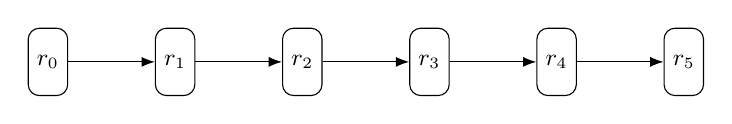
\begin{tikzpicture}[>=Latex,box/.style={draw,rounded corners,align=center,minimum height=9mm,font=\small},scale=0.95,transform shape]
\node[box] (r0) at (0.0,0) {$r_0$};
\node[box] (r1) at (1.7,0) {$r_1$};
\node[box] (r2) at (3.4,0) {$r_2$};
\node[box] (r3) at (5.1,0) {$r_3$};
\node[box] (r4) at (6.8,0) {$r_4$};
\node[box] (r5) at (8.5,0) {$r_5$};
\draw[->] (r0) -- (r1);
\draw[->] (r1) -- (r2);
\draw[->] (r2) -- (r3);
\draw[->] (r3) -- (r4);
\draw[->] (r4) -- (r5);
\end{tikzpicture}\end{center}

\sol The drawing does not state a seed, so assume a cleared register.
Number stages $r_0,\ldots,r_5$ from input to output and read the outgoing
$r_5$ \emph{before} each shift. No extra flush clocks are applied.
All sums below are XORs over $\mathrm{GF}(2)$.

For the distributed-feedback circuit, let $f=r_5$.
First form $(r_0',\ldots,r_5')=(u,r_0,r_1,r_2,r_3,r_4)$,
then XOR $f$ into positions $\{0,3,4,5\}$.
For the input-feedback circuit,
\[
r_0'=u+r_0+r_1+r_2+r_5,\qquad r_i'=r_{i-1}\quad(1\le i\le5).
\]
These recurrences, rather than a visually reversed polynomial label, define
the bit ordering unambiguously.
\begin{center}\begin{tabular}{lll}\toprule
Circuit & Serial output, first bit first & Final $(r_0,\ldots,r_5)$\\\midrule
Distributed & \texttt{00000011110100000100100} & \texttt{101001}\\
Input feedback & \texttt{00000011110100000100100} & \texttt{001011}\\
\bottomrule\end{tabular}\end{center}
The first six outgoing bits are the initial zero state.
Deleting that six-bit latency gives the emitted quotient portion during the
remaining input clocks. The table gives physical register signatures;
Fibonacci and distributed-feedback state encodings differ although their
outgoing streams agree. Reversing the signature, clocking six extra zeros or
using a nonzero seed changes the printed result and must be stated.

\section{IEEE 1149.1 interconnect testing}
\textbf{Question.} Three ICs form the serial chain
$TDI\to IC1\to IC2\to IC3\to TDO$.
The four lines $X_1,\ldots,X_4$ run from IC1 outputs to IC2 inputs.
Describe the instructions and patterns required to detect
both stuck-at values of interconnects $X_1,\ldots,X_4$.\begin{center}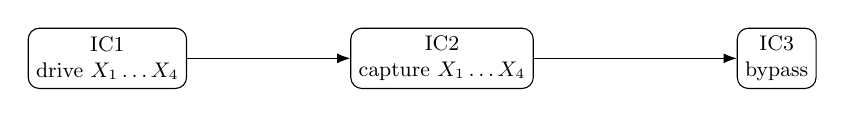
\begin{tikzpicture}[>=Latex,box/.style={draw,rounded corners,align=center,minimum height=9mm,font=\small},scale=0.85,transform shape]
\node[box] (i1) at (0,0) {IC1\\drive $X_1\ldots X_4$};
\node[box] (i2) at (5,0) {IC2\\capture $X_1\ldots X_4$};
\node[box] (i3) at (10,0) {IC3\\bypass};
\draw[->] (i1) -- (i2);
\draw[->] (i2) -- (i3);
\end{tikzpicture}\end{center}

\sol Put IC1 and IC2 in EXTEST; put the uninvolved IC3 in BYPASS.
Preload safe drive values, update the launch cells, allow interconnect settling,
capture at IC2, then shift out the captured response. Drive 1111 to detect SA0;
drive 0000 to detect SA1. Other boundary cells must have safe values, especially
output enables, to prevent contention.

\paragraph{1149.1 versus 1500.}
IEEE 1149.1 primarily gives chip/board boundary access through a TAP controller
and a standardized serial state machine. IEEE 1500 wraps embedded cores inside
an SoC; it separates the wrapper from the system-level test access mechanism
and supports wrapper serial access with optional parallel access for bandwidth.
Thus their intended integration level and access/control architecture differ.
See the TI boundary-scan design note and IEEE 1500 standard overview linked in
\texttt{exams/README.md}.

\section{Full-scan conversion and stuck-at tests}
\textbf{Question.} Convert the sequential circuit to full scan, derive tests
covering all stuck-at faults of the combinational logic, and describe the
application sequence. The reconstructed normal-mode netlist is:
\begin{center}\begin{tabular}{ll}\toprule Signal & Defining expression\\\midrule
$g_1$ & $\overline{X_2\oplus Q_1}$\\
$g_2$ & $\overline{g_1\oplus Q_2}$\\
$h$ & $\overline{g_2\oplus Q_3}$\\
$Y$ & $X_1+h$\\
$D_1$ & $g_2$\\
$D_2$ & $h$\\
$D_3$ & $g_1$\\
\bottomrule\end{tabular}\end{center}
\begin{center}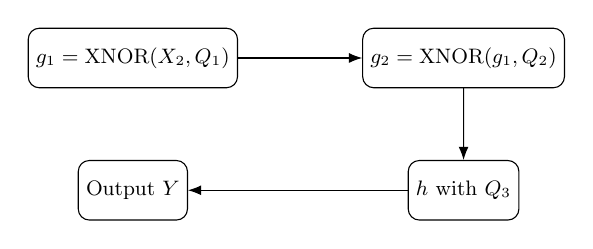
\begin{tikzpicture}[>=Latex,box/.style={draw,rounded corners,align=center,minimum height=9mm,font=\small},scale=0.84,transform shape]
\node[box] (g1) at (0,0) {$g_1=\operatorname{XNOR}(X_2,Q_1)$};
\node[box] (g2) at (5,0) {$g_2=\operatorname{XNOR}(g_1,Q_2)$};
\node[box] (h) at (5,-2) {$h$ with $Q_3$};
\node[box] (y) at (0,-2) {Output $Y$};
\draw[->] (g1) -- (g2);
\draw[->] (g2) -- (h);
\draw[->] (h) -- (y);
\end{tikzpicture}\end{center}

\sol Replace every D flip-flop by a muxed scan flip-flop:
$D_i^{\rm scan}=SE?SI_i:D_i$.
Connect $SI\to FF_1\to FF_2\to\cdots\to FF_n\to SO$ with common scan enable
and a controllable clock. Scan state outputs are independent pseudo-inputs;
all functional D inputs become observable pseudo-outputs.
\begin{center}\begin{tabular}{lll}\toprule $(X_1,X_2,Q_1,\ldots,Q_n)$ & $(D_1,\ldots,D_n)$ & $Y$\\\midrule
00001 & 001 & 0\\
00101 & 110 & 1\\
11110 & 101 & 1\\
\bottomrule\end{tabular}\end{center}
Exhaustive enumeration of all $2^{5}$ input assignments verifies
46/46 single stuck-at faults for this netlist:
both values on every signal stem and on every individual gate-input branch.
Identity buffers at the observed D pins also model their separate output branches.
No modeled faults are redundant. The displayed set is sufficient, not claimed minimum.

For each row: assert $SE=1$; shift $Q_n,\ldots,Q_1$ in that order;
set $X_1,X_2$; deassert $SE$ and observe $Y$ before the capture edge;
apply one functional capture clock; reassert $SE$ and unload
$D_n,\ldots,D_1$ while loading the next state.
Account for scan-in/out bit order and compare only the expected response positions.
The proof covers combinational SAFs, not all scan-mux, clock, reset or analog defects.

\section{Defects in a two-by-two SRAM}
\textbf{Question.} A $2\times2$ bit-oriented SRAM has defect $d_1$ across a
cell's access transistor and defect $d_2$ in a pull-up connection.
Identify the faults and develop a March test for $d_2$.
\textbf{Source-reading note.} The scan shows $d_1$ as a bypass/bridge across
the left access device of cell $(0,0)$, and $d_2$ as an open in the right
pull-up path of cell $(0,1)$. The interpretation below states this explicitly.
\begin{center}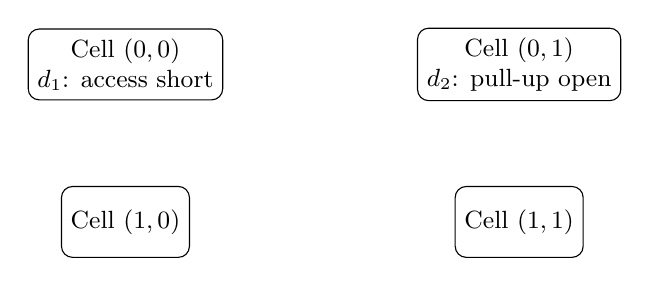
\begin{tikzpicture}[>=Latex,box/.style={draw,rounded corners,align=center,minimum height=9mm,font=\small},scale=1,transform shape]
\node[box] (a) at (0,0) {Cell $(0,0)$\\$d_1$: access short};
\node[box] (b) at (5,0) {Cell $(0,1)$\\$d_2$: pull-up open};
\node[box] (c) at (0,-2) {Cell $(1,0)$};
\node[box] (d) at (5,-2) {Cell $(1,1)$};
\end{tikzpicture}\end{center}

\sol $d_1$ makes the cell permanently coupled to its bitline even when its
wordline is not selected. It can cause read/write disturbance or coupling
between cells sharing the column; a unique single-cell stuck-at label cannot
be justified without bitline/precharge and strength assumptions.
$d_2$ removes a restoring pull-up path. A write can initially charge the
affected node, but leakage may then destroy one stored polarity: a
data-retention/stuck-open fault, rather than necessarily a static SAF.

Use a retention-extended March sequence, testing both data polarities:
\[
\{\any(w0);\ \mathrm{wait}(t_R);\ \any(r0,w1);\
  \mathrm{wait}(t_R);\ \any(r1,w0)\}.
\]
Every cell must wait at least $t_R$ after its own write and before its read.
A global wait after an all-cell write guarantees that lower bound.
Choose $t_R$ from the SRAM retention specification; no value is supplied in
the exam. The first read phase catches loss of 0; the second catches loss of 1.
An immediate read after a write can miss the open pull-up because the
node may temporarily retain its capacitive charge.

\section{IEEE 1500 wrapper external test}
\textbf{Question.} A wrapped core has two internal scan chains, a wrapper
boundary register (WBR), a wrapper instruction register and a bypass register.
(a) For an ExTestS serial external test, describe the data path and application.
(b) Modify the architecture to support an ExTestP parallel external test with
reduced test time.
\begin{center}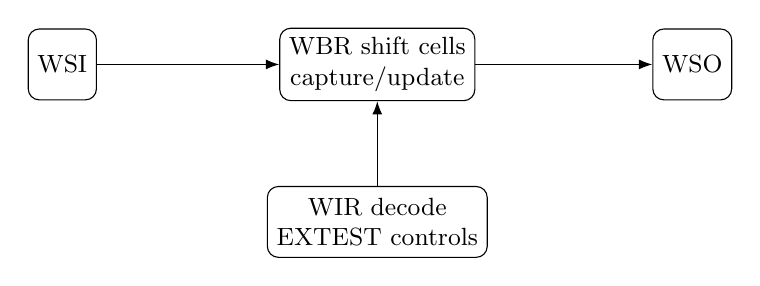
\begin{tikzpicture}[>=Latex,box/.style={draw,rounded corners,align=center,minimum height=9mm,font=\small},scale=1,transform shape]
\node[box] (wsi) at (0,0) {WSI};
\node[box] (wbr) at (4,0) {WBR shift cells\\capture/update};
\node[box] (wso) at (8,0) {WSO};
\node[box] (wir) at (4,-2) {WIR decode\\EXTEST controls};
\draw[->] (wsi) -- (wbr);
\draw[->] (wbr) -- (wso);
\draw[->] (wir) -- (wbr);
\end{tikzpicture}\end{center}

\sol Shift the ExTestS instruction through the wrapper instruction path and update
the instruction latch. Select the boundary register, bypassing core-internal
scan chains for this external test. The serial test-data path is
WSI$\to$WBR cells around the core$\to$WSO.
Shift known values into source-side boundary cells, perform UpdateWR to launch
them into the interconnect/glue logic, allow settling, capture receiving-side
boundary responses with CaptureWR and shift them out with ShiftWR.
Instruction bits are control, not inserted into every external-test data word.

For ExTestP, provide a wrapper parallel port and a TAM of width $w$,
partition the active boundary cells into $w$ accessible segments, and add
mode-controlled input/output selection to connect each segment to a lane.
Balance segment lengths, retain capture/update behavior and preserve serial
access for setup and compatibility. With total $N$ shifted bits, the ideal
shift count changes from $N$ to roughly $\lceil N/w\rceil$, subject to the
longest actual segment and fixed control overhead. Simply adding an opcode
without parallel data routing does not reduce time.

\end{document}
